\documentclass[11pt]{article}
\usepackage[margin=1in]{geometry}
\usepackage{amsmath,amssymb,amsthm}
\usepackage[T1]{fontenc}
\usepackage{lmodern}
\usepackage{graphicx}
\usepackage[hidelinks]{hyperref}
\usepackage{xcolor}

\newtheorem{theorem}{Theorem}
\newtheorem{lemma}[theorem]{Lemma}
\newtheorem{remark}[theorem]{Remark}
\newcommand{\R}{\mathbb R}
\newcommand{\T}{\mathbb T}
\newcommand{\B}{\mathcal B}
\newcommand{\spec}{\operatorname{spec}}

\title{The Sharp Scaled Limsup Law for Cosine Families}
\author{Full literature-implied answer to arXiv:1310.6202}
\date{11 August 2026}

\begin{document}
\maketitle

\begin{center}
\fcolorbox{black}{gray!8}{\parbox{0.88\linewidth}{
\textbf{Status: literature-implied answer, full scope, likely valid.}
The scaled cosine question has a sharp affirmative answer.  For $a>0$ the
optimal constant is $8/(3\sqrt3)$; for $a=0$ it is $2$.  The semigroup
constant is $1$.  The scaled conclusion follows by combining two theorems of
Esterle with a recurrence observation; the supporting authors did not state
this limsup implication and a later paper still listed it as open.}}
\end{center}

\section{Source question}

Schwenninger and Zwart prove that a strongly continuous cosine family
$(C(t))_{t\geq0}$ on a Banach space satisfies
\[
 \sup_{t\geq0}\|C(t)-\cos(at)I\|<1
 \quad\Longrightarrow\quad C(t)=\cos(at)I.
\]
Their final Remark 2.6 asks whether the supremum can be replaced by
\[
 \limsup_{t\to\infty}\|C(t)-\cos(at)I\|<1,
\]
or even by a bound with a constant larger than $1$.  It also says that the
semigroup analogue was unclear \cite{SZ13}.

\begin{figure}[ht]
  \centering
  
\includegraphics[width=\textwidth]{figures/open_question_crop.png}
  \caption{Remark 2.6 in arXiv:1310.6202v3, PDF page 6.}
\end{figure}

The answer below is stronger and sharp.  The relation to the supporting
literature is an implication identified here: arXiv:1504.02355 explicitly
settles the unscaled and semigroup cases, while arXiv:1502.00150 supplies the
two structural theorems that settle the remaining scaled case.
\clearpage

\section{Supporting results}

We use two results from Esterle \cite{E15}.

\begin{enumerate}
\item Theorem 2.3: if $(c_n)_{n\in\mathbb Z}$ is a bounded cosine sequence
in a Banach algebra and $\spec(c_1)$ is a singleton, then the sequence is
scalar: $c_n=\cos(nb)1$ for some $b\in\R$.
\item Lemma 3.5(ii): for $a\geq0$, if
\[
 \sup_{t\in\R}|\cos(at)-\cos(bt)|<\frac{8}{3\sqrt3},
\]
then $b=a$.  The constant is optimal for $a>0$, since
\[
 \sup_t|\cos(at)-\cos(3at)|=\frac{8}{3\sqrt3}.
\]
\end{enumerate}

\begin{figure}[ht]
  \centering
  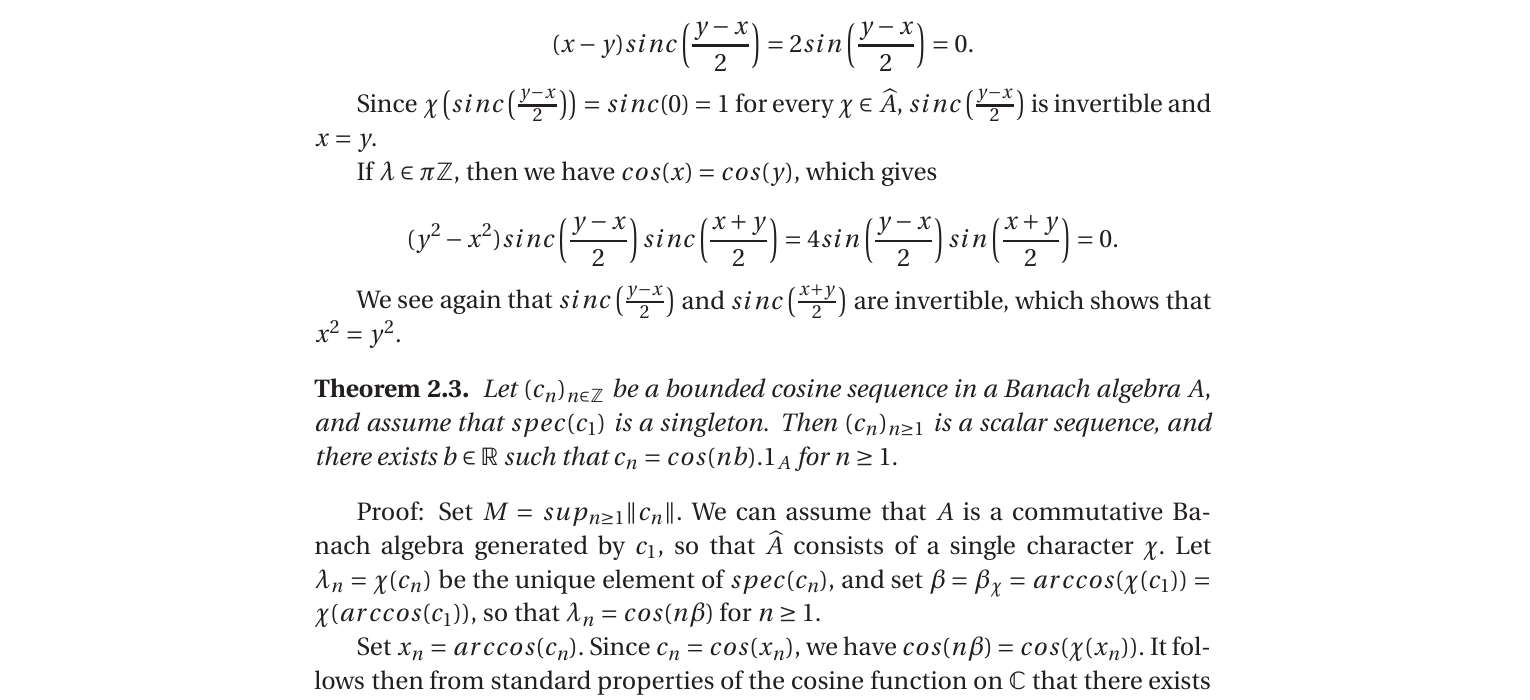
\includegraphics[width=\textwidth]{figures/singleton_theorem_crop.png}
  \caption{Esterle's singleton-spectrum rigidity theorem,
  arXiv:1502.00150v2, PDF page 6.}
\end{figure}

\begin{figure}[ht]
  \centering
  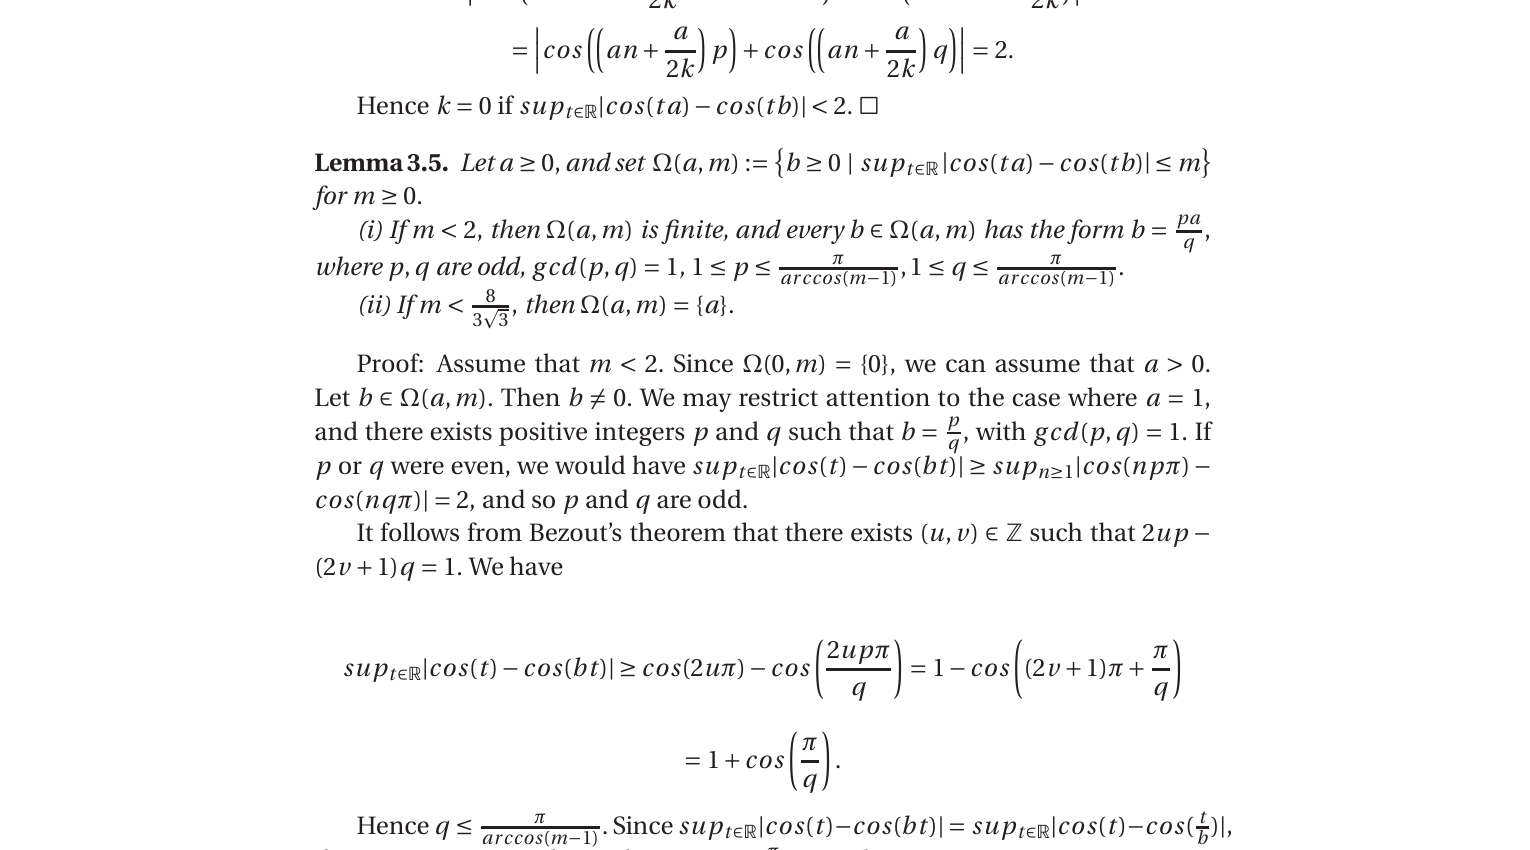
\includegraphics[width=\textwidth]{figures/scalar_separation_crop.png}
  \caption{Esterle's sharp scalar separation lemma,
  arXiv:1502.00150v2, PDF page 9.}
\end{figure}
\clearpage

\section{The sharp answer}

\begin{theorem}[Sharp scaled limsup law]\label{thm:main}
Let $(C(t))_{t\in\R}$ be a strongly continuous cosine family on a complex
Banach space $X$.

\begin{enumerate}
\item If $a>0$ and
\[
 L:=\limsup_{t\to\infty}\|C(t)-\cos(at)I\|
 <\frac{8}{3\sqrt3},
\]
then $C(t)=\cos(at)I$ for every $t\in\R$.
The constant $8/(3\sqrt3)$ is optimal.

\item If $a=0$ and
\[
 \limsup_{t\to\infty}\|C(t)-I\|<2,
\]
then $C(t)=I$ for every $t\in\R$, and $2$ is optimal.
\end{enumerate}
\end{theorem}

\begin{proof}
The second assertion is exactly Theorem 2.5 of Schwenninger--Zwart
\cite{SZ15}; optimality follows from any nonconstant scalar cosine.

We prove the first assertion.  The tail hypothesis bounds $C(t)$ for all
sufficiently large $t$.  Strong continuity and the uniform boundedness
principle bound it on each compact interval, while $C(-t)=C(t)$.  Hence
\[
 M:=\sup_{t\in\R}\|C(t)\|<\infty.
\]
Let $A$ be the closed unital subalgebra of $\B(X)$ generated by the family.
The cosine identity makes $A$ commutative.  Fix a character $\chi$ of $A$.
Then
\[
 c_\chi(t):=\chi(C(t))
\]
is a bounded scalar cosine function.

We first note a standard scalar dichotomy.  If a bounded scalar cosine
function $c$ on $\R$ is discontinuous, then for every continuous scalar
cosine $t\mapsto\cos(at)$,
\begin{equation}\label{eq:disc}
 \limsup_{t\to\infty}|c(t)-\cos(at)|=2.
\end{equation}
One way to see this is to write
$c(t)=(\gamma(t)+\gamma(t)^{-1})/2$ for a group character
$\gamma:\R\to\T$.  If the closure of
$t\mapsto(e^{iat},\gamma(t))$ is a proper subgroup of $\T^2$, an integer
relation makes a nonzero power of $\gamma$ continuous; divisibility of
$\R$ then makes $\gamma$ continuous.  Otherwise the image is dense in
$\T^2$.  The same is true on every positive tail, by recurrence in the
compact group, and \eqref{eq:disc} follows.  For $a=0$ the identical
argument uses only the second coordinate.  This is also the
infinity-tail counterpart of Esterle's discontinuous-scalar density
proposition \cite[Proposition 3.1]{E15}.

Since
\[
 \limsup_{t\to\infty}|c_\chi(t)-\cos(at)|
 \leq L<2,
\]
the dichotomy shows that $c_\chi$ is continuous.  Thus
$c_\chi(t)=\cos(b_\chi t)$ for some $b_\chi\geq0$.  A finite sum of
continuous scalar characters is recurrent, so
\[
 \sup_{t\in\R}|\cos(b_\chi t)-\cos(at)|
 =\limsup_{t\to\infty}|\cos(b_\chi t)-\cos(at)|
 \leq L.
\]
Esterle's Lemma 3.5(ii) now gives $b_\chi=a$.  Therefore, for every
$s\in\R$ and every character $\chi$,
\[
 \chi(C(s))=\cos(as),
\]
and hence
\begin{equation}\label{eq:singleton}
 \spec_A(C(s))=\{\cos(as)\}.
\end{equation}

Fix $s$.  The sampled family $c_n=C(ns)$ is a bounded cosine sequence in
$A$, and its first element has singleton spectrum by
\eqref{eq:singleton}.  Esterle's Theorem 2.3 says that this sequence is
scalar.  In particular $C(s)$ is scalar, and its unique spectral value in
\eqref{eq:singleton} forces
\[
 C(s)=\cos(as)I.
\]
Since $s$ was arbitrary, the desired identity holds on all of $\R$.

Finally, when $a>0$, the scalar cosine family
$C(t)=\cos(3at)I$ is nontrivial and has limsup distance exactly
$8/(3\sqrt3)$.  Thus no larger strict-threshold constant is possible.
\end{proof}

\begin{theorem}[Sharp semigroup limsup law]
Let $(T(t))_{t\geq0}$ be a semigroup in a unital normed algebra.  Then
\[
 \limsup_{t\to\infty}\|T(t)-I\|<1
 \quad\Longrightarrow\quad T(t)=I\quad(t\geq0).
\]
The constant $1$ is optimal.
\end{theorem}

\begin{proof}
This is Theorem 3.1 and Remark 3.2 of Schwenninger--Zwart \cite{SZ15}.
Sharpness is witnessed by the scalar semigroup $T(t)=e^{-t}$, for which the
limsup distance is $1$.
\end{proof}

\begin{figure}[ht]
  \centering
  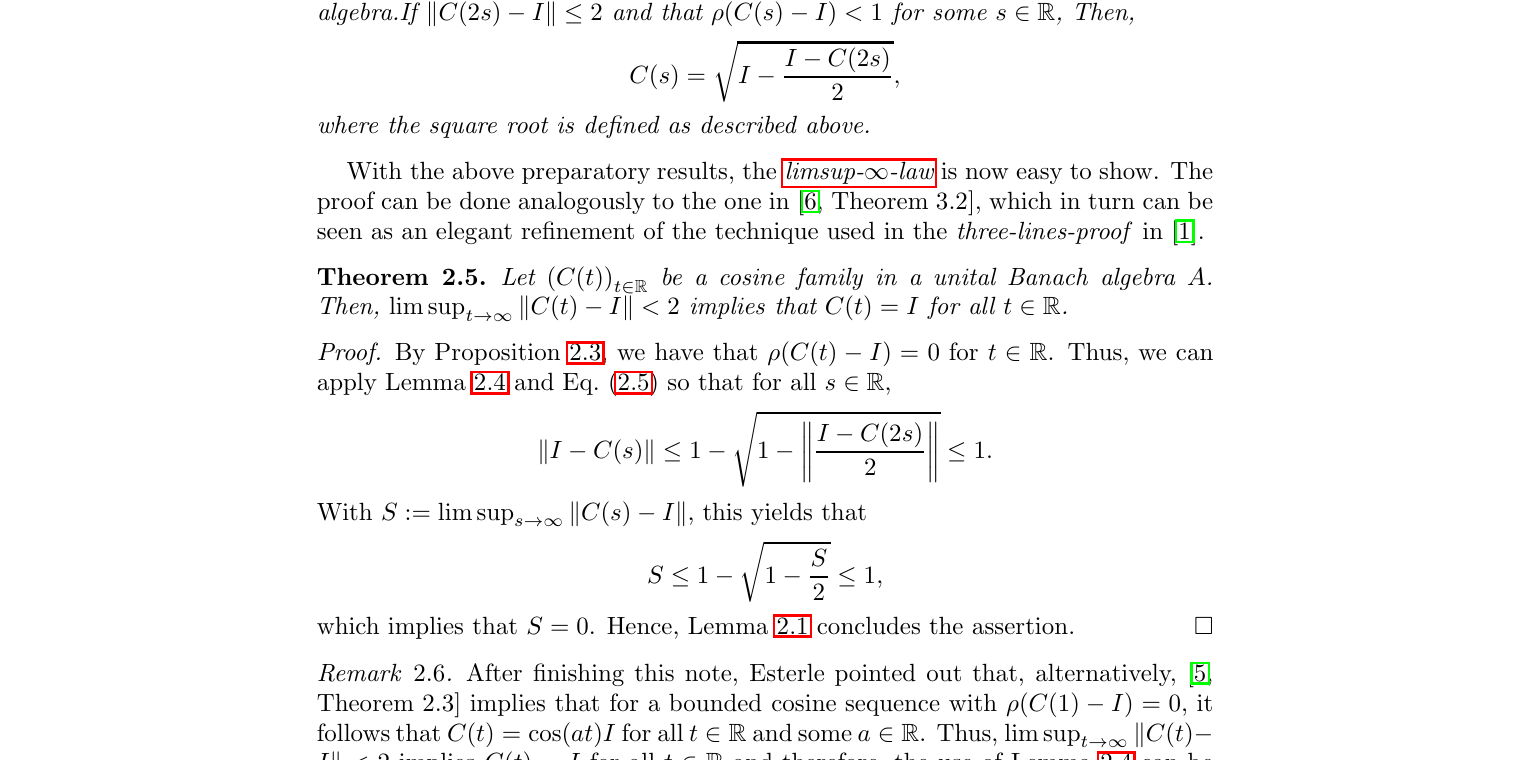
\includegraphics[width=\textwidth]{figures/zero_two_crop.png}
  \caption{The sharp unscaled cosine result, arXiv:1504.02355v1,
  PDF page 3.}
\end{figure}

\begin{figure}[ht]
  \centering
  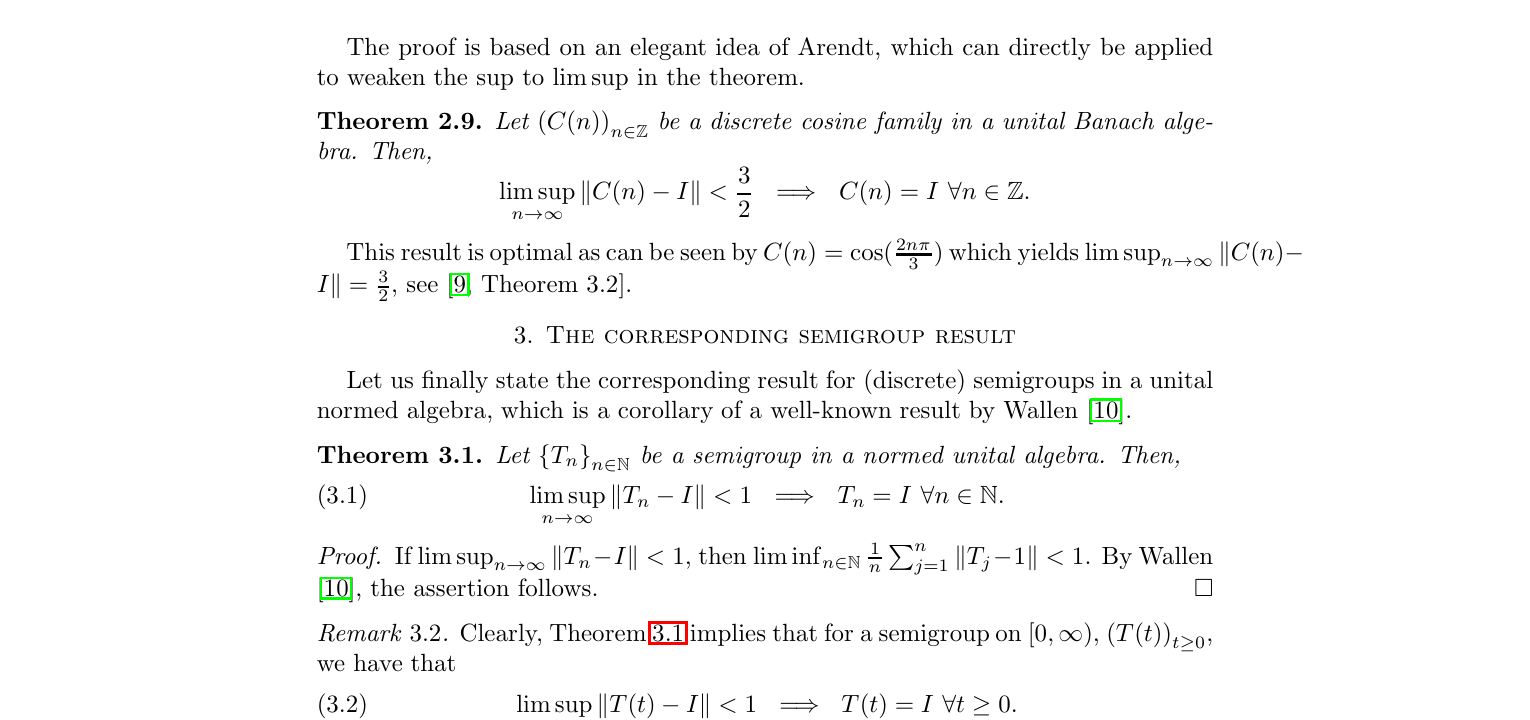
\includegraphics[width=\textwidth]{figures/semigroup_crop.png}
  \caption{The semigroup limsup result, arXiv:1504.02355v1,
  PDF page 4.}
\end{figure}
\clearpage

\section{Status, scope, and search bounds}

This settles every case mentioned in Remark 2.6, and it gives the best
possible constants.  The provenance is \emph{literature-implied}, not an
explicit later answer: Schwenninger--Zwart \cite{SZ15} explicitly settle
$a=0$ and semigroups, but still describe the scaled law as a related open
question.  Esterle \cite{E15} proves the two decisive ingredients, but does
not state their tail-limsup consequence.  The short character-spectrum
bridge in the proof above identifies that consequence.

A bounded search used the exact formula, the source id and title, author
names, and the phrases ``scaled cosine family'', ``limsup to infinity'',
and ``scalar cosine family''.  It found arXiv:1504.02355,
arXiv:1502.00150, and arXiv:1505.06064 (the discrete-group analogue), but
no later paper explicitly stating the continuous scaled limsup theorem.
Novelty is therefore claimed only for the identification, not for the two
supporting structural theorems.

Human review should focus on the scalar discontinuity dichotomy
\eqref{eq:disc} and on applying Esterle's Theorem 2.3 inside the generated
commutative Banach algebra.  Both remaining steps are direct.

\begin{thebibliography}{9}
\bibitem{SZ13}
F. L. Schwenninger and H. Zwart,
\emph{Less than one implies zero}, arXiv:1310.6202v3 (2015).

\bibitem{E15}
J. Esterle,
\emph{Bounded cosine functions close to continuous scalar bounded cosine
functions}, arXiv:1502.00150v2 (2015).

\bibitem{SZ15}
F. L. Schwenninger and H. Zwart,
\emph{A $0$--$2$ law for cosine families with $\limsup$ to infinity},
arXiv:1504.02355v1 (2015).
\end{thebibliography}

\end{document}
